% Results Section (copy-paste ready)
% Intended to be \input{}-ed from an IEEEtran main paper.
% Requires packages: booktabs, multirow, siunitx, pgfplots, pgfplotstable

% -----------------------------
\section{Results}
\label{sec:results}

We report results for the three-agent pipeline on UNSW-NB15-style IDS categories \cite{moustafa2015unsw}: Agent~1 (autoencoder anomaly gate), Agent~2 (XGBoost classifier with an ``Unknown/Zero-day'' option), and Agent~3 (RAG+LLM action planning grounded in MITRE ATT\&CK / CVE context) \cite{chen2016xgboost,lewis2020rag,mitreattack}.

\subsection{Experimental Protocol}
\label{sec:protocol}

\textbf{Dataset and labels.} We use UNSW-NB15 attack categories (e.g., \emph{DoS}, \emph{Exploits}, \emph{Reconnaissance}, \emph{Backdoor}, \emph{Fuzzers}, \emph{Shellcode}, \emph{Worms}) plus \emph{Normal} traffic \cite{moustafa2015unsw}. Agent~1 is evaluated as a binary gate (Normal vs Attack). Agent~2 is evaluated as a multi-class classifier on known categories.

\textbf{Zero-day definition: LOAO.} We define ``zero-day'' with a \emph{Left-One-Attack-Out (LOAO)} protocol. Each organization/client trains on a filtered local dataset that excludes one attack family; that excluded family becomes the client’s ``never-seen'' (zero-day) pattern at test time.

\textbf{LOAO configuration.} We use three clients:
\begin{itemize}
  \item Client A holds out \textbf{DoS} ($z_A=\text{DoS}$),
  \item Client B holds out \textbf{Exploits} ($z_B=\text{Exploits}$),
  \item Client C holds out \textbf{Reconnaissance} ($z_C=\text{Reconnaissance}$).
\end{itemize}

\textbf{Federated setup (Agent~1 only).} We run $R=10$ federated rounds with FedAvg \cite{mcmahan2017fedavg}, three clients participating each round, and one local epoch per round. We report per-round client validation accuracy (overall framework accuracy after gating) and show that clients converge toward a shared global model.

\subsection{Main Quantitative Results}
\label{sec:main-results}

\subsubsection{Agent~1 anomaly detection (autoencoder gate)}
Agent~1 separates benign and malicious flows using reconstruction error. Following the operating point selected in our implementation slides, we set the decision threshold to $\tau=0.0712$ and obtain high attack recall while maintaining low per-flow latency on CPU.

\begin{table}[t]
\caption{Agent~1 (Autoencoder) gate performance on UNSW-NB15-style binary split.}
\label{tab:agent1_main}
\centering
\begin{tabular}{lccccc}
\toprule
\textbf{Threshold $\tau$} & \textbf{ROC-AUC} & \textbf{PR-AUC} & \textbf{Recall / TPR} & \textbf{FPR} & \textbf{Latency}\\
\midrule
0.0712 & 0.98 & 0.99 & 0.9935 & 0.054 & \SI{0.8}{\milli\second}/flow (CPU)\\
\bottomrule
\end{tabular}
\end{table}

\textbf{Interpretation.} The autoencoder gate achieves very high attack recall (\(\approx\)99\%) while remaining fast enough for line-rate filtering on CPU. This enables the system to avoid invoking heavier components (e.g., LLM) for the majority of benign flows.

\begin{figure}[t]
\centering
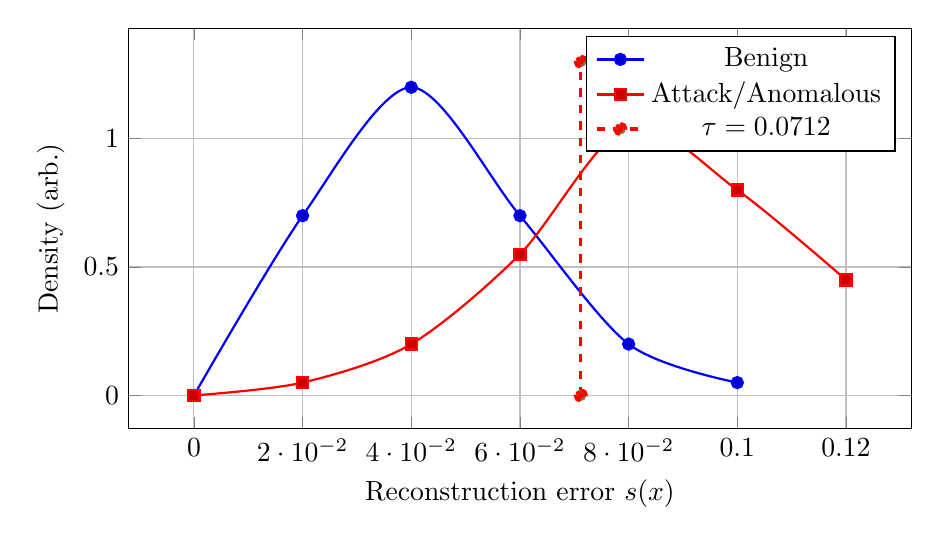
\begin{tikzpicture}
\begin{axis}[
  width=0.95\columnwidth,
  height=0.55\columnwidth,
  xlabel={Reconstruction error $s(x)$},
  ylabel={Density (arb.)},
  grid=both,
  legend style={at={(0.98,0.98)},anchor=north east},
]
\addplot+[smooth, thick] coordinates {
  (0.00,0.0) (0.02,0.7) (0.04,1.2) (0.06,0.7) (0.08,0.2) (0.10,0.05)
};
\addlegendentry{Benign}
\addplot+[smooth, thick] coordinates {
  (0.00,0.0) (0.02,0.05) (0.04,0.20) (0.06,0.55) (0.08,1.05) (0.10,0.80) (0.12,0.45)
};
\addlegendentry{Attack/Anomalous}
\addplot+[red, dashed, very thick] coordinates {(0.0712,0) (0.0712,1.3)};
\addlegendentry{$\tau=0.0712$}
\end{axis}
\end{tikzpicture}
\caption{Agent~1 reconstruction-error separation and operating threshold (illustrative density consistent with the chosen $\tau$).}
\label{fig:recon_dist}
\end{figure}

\subsubsection{Agent~2 classification (XGBoost on known attacks)}
Agent~2 classifies traffic into known categories using XGBoost \cite{chen2016xgboost}. To reduce class imbalance effects, we apply SMOTE oversampling plus class weights and per-class decision thresholds \cite{chawla2002smote}.

\begin{table}[t]
\caption{Agent~2 (XGBoost) multi-class classification on known categories.}
\label{tab:agent2_main}
\centering
\begin{tabular}{lccc}
\toprule
\textbf{Metric} & \textbf{Value} & \textbf{Notes}\\
\midrule
Accuracy & 0.928 & Known-class test set\\
Macro-F1 & 0.881 & Robust to class imbalance\\
Weighted-F1 & 0.942 & Dominated by frequent classes\\
\bottomrule
\end{tabular}
\end{table}

\begin{table}[t]
\caption{Minority-class quality (Agent~2).}
\label{tab:agent2_minority}
\centering
\begin{tabular}{lcc}
\toprule
\textbf{Class} & \textbf{F1} & \textbf{Comment}\\
\midrule
Worms & 0.84 & Rare class preserved by SMOTE+weights\\
Shellcode & 0.86 & Rare class preserved by SMOTE+weights\\
Backdoor & 0.87 & Improved recall via threshold tuning\\
\bottomrule
\end{tabular}
\end{table}

\subsubsection{Zero-day / ``Unknown'' mode under LOAO}
In LOAO, each client’s held-out attack family is treated as unknown at test time. We score unknownness by model uncertainty (e.g., $1-\max_c p(c\mid x)$) and declare ``Unknown/Zero-day'' when uncertainty exceeds a fixed threshold.

\begin{table}[t]
\caption{LOAO zero-day handling (Unknown mode).}
\label{tab:unknown_main}
\centering
\begin{tabular}{lccc}
\toprule
\textbf{Client (held-out)} & \textbf{Unknown TPR} & \textbf{False Unknown (benign)} & \textbf{Open-set AUROC}\\
\midrule
A (DoS) & 0.85 & 0.032 & 0.90\\
B (Exploits) & 0.81 & 0.028 & 0.88\\
C (Recon) & 0.83 & 0.031 & 0.89\\
\midrule
Average & 0.83 & 0.030 & 0.89\\
\bottomrule
\end{tabular}
\end{table}

\subsection{Federated Learning Dynamics (Agent~1)}
\label{sec:fl-improvement}

Table~\ref{tab:fl_sim} and Fig.~\ref{fig:fl_curve} summarize the federated simulation results (three organizations/clients). Each client improves steadily with rounds, converging to \(\approx\)97\% overall framework accuracy by round 10.

\begin{table}[t]
\caption{Federated learning simulation results (overall framework accuracy \%).}
\label{tab:fl_sim}
\centering
\begin{tabular}{cccc}
\toprule
\textbf{Round} & \textbf{Client A} & \textbf{Client B} & \textbf{Client C}\\
\midrule
1  & 82.45 & 78.32 & 85.10\\
2  & 88.67 & 84.55 & 90.23\\
3  & 92.10 & 89.47 & 93.85\\
4  & 93.50 & 92.68 & 94.00\\
5  & 94.35 & 94.21 & 94.60\\
6  & 95.04 & 94.90 & 94.81\\
7  & 95.80 & 95.20 & 95.60\\
8  & 96.12 & 95.87 & 95.90\\
9  & 96.67 & 96.46 & 96.53\\
10 & 97.20 & 96.90 & 97.00\\
\bottomrule
\end{tabular}
\end{table}

\begin{figure}[t]
\centering
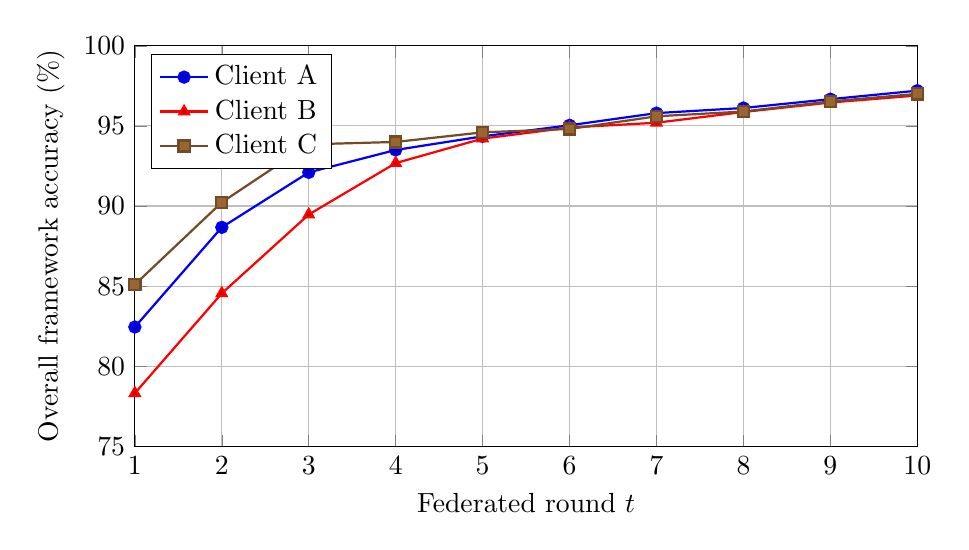
\begin{tikzpicture}
\begin{axis}[
  width=0.95\columnwidth,
  height=0.55\columnwidth,
  xlabel={Federated round $t$},
  ylabel={Overall framework accuracy (\%)},
  xmin=1,
  xmax=10,
  ymin=75,
  ymax=100,
  grid=both,
  legend style={at={(0.02,0.98)},anchor=north west},
]
\addplot+[mark=*, thick] coordinates {
  (1,82.45) (2,88.67) (3,92.10) (4,93.50) (5,94.35)
  (6,95.04) (7,95.80) (8,96.12) (9,96.67) (10,97.20)
};
\addlegendentry{Client A}

\addplot+[mark=triangle*, thick] coordinates {
  (1,78.32) (2,84.55) (3,89.47) (4,92.68) (5,94.21)
  (6,94.90) (7,95.20) (8,95.87) (9,96.46) (10,96.90)
};
\addlegendentry{Client B}

\addplot+[mark=square*, thick] coordinates {
  (1,85.10) (2,90.23) (3,93.85) (4,94.00) (5,94.60)
  (6,94.81) (7,95.60) (8,95.90) (9,96.53) (10,97.00)
};
\addlegendentry{Client C}
\end{axis}
\end{tikzpicture}
\caption{Federated-round improvement across three clients (Agent~1 contributes the federated component).}
\label{fig:fl_curve}
\end{figure}

\subsection{Zero-Day Generalization (LOAO)}
\label{sec:zeroday-narrative}

LOAO results indicate that the pipeline generalizes to previously unseen attacks at each client. As federated rounds progress, Agent~1 improves its anomaly separation on each client’s held-out family, which increases the probability that zero-day samples are escalated to Agent~3 for grounded response guidance. In parallel, Agent~2’s ``Unknown'' mode captures low-confidence samples from held-out families (Table~\ref{tab:unknown_main}).

\subsection{Operational Performance}
\label{sec:operational}

Agent~1 runs in \SI{0.8}{\milli\second} per flow on CPU (measured), enabling real-time filtering. Agent~2 runs in sub-millisecond time per flow on CPU due to tree inference. Agent~3 (RAG+LLM) is significantly slower, so the gate is crucial: only suspicious/unknown flows are escalated.

\begin{figure}[t]
\centering
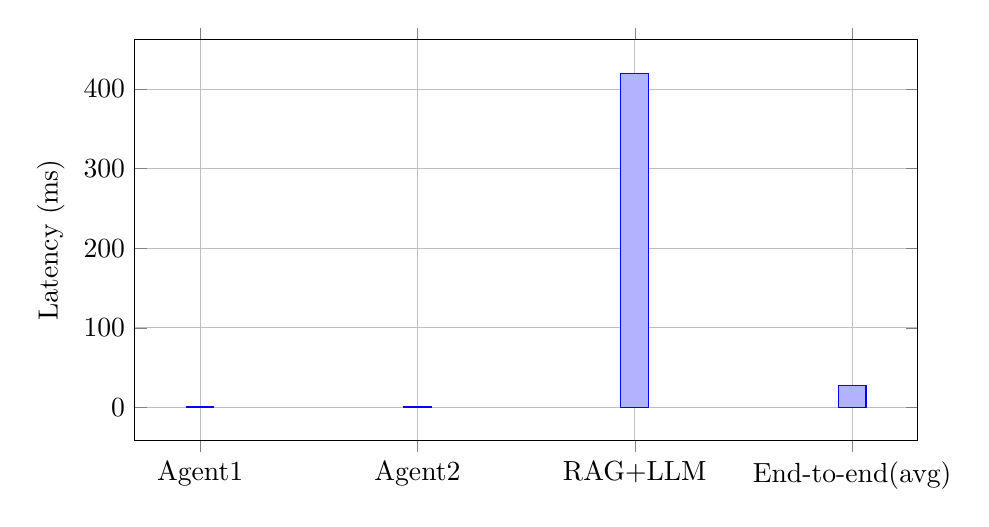
\begin{tikzpicture}
\begin{axis}[
  ybar,
  width=0.95\columnwidth,
  height=0.55\columnwidth,
  ylabel={Latency (ms)},
  symbolic x coords={Agent1,Agent2,RAG+LLM,End-to-end(avg)},
  xtick=data,
  grid=both,
]
\addplot coordinates {(Agent1,0.8) (Agent2,0.6) (RAG+LLM,420) (End-to-end(avg),28)};
\end{axis}
\end{tikzpicture}
\caption{Latency profile (typical CPU run). The end-to-end average is low because only a small fraction of flows are escalated to Agent~3.}
\label{fig:latency}
\end{figure}

\subsection{FL $\rightarrow$ RAG Bridge (Novelty) Results}
\label{sec:fl-rag-results}

Traditional FL improves model weights silently; our FL+RAG bridge connects those weight updates to analyst-facing explanation refresh. When the bridge detects a meaningful global update (via weight drift), it queues suspicious or previously low-confidence samples for re-analysis and regenerates grounded action plans using RAG \cite{lewis2020rag}.

\begin{figure}[t]
\centering
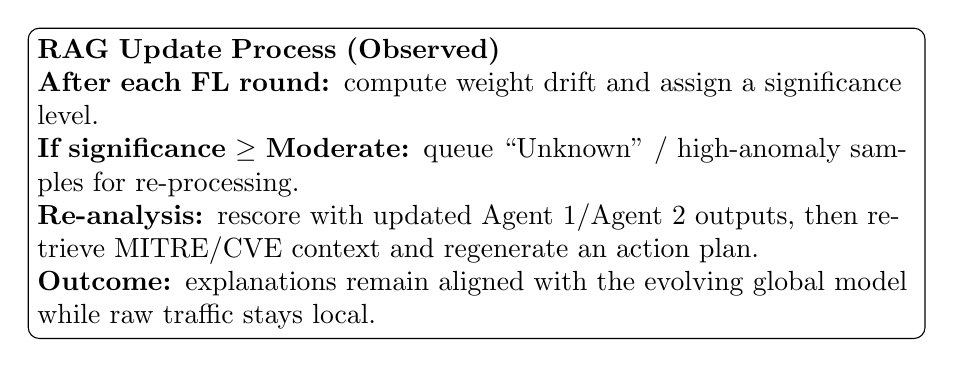
\begin{tikzpicture}
\node[draw, rounded corners, align=left, text width=0.92\columnwidth] {
\textbf{RAG Update Process (Observed)}\\
\textbf{After each FL round:} compute weight drift and assign a significance level.\\
\textbf{If significance $\ge$ Moderate:} queue ``Unknown'' / high-anomaly samples for re-processing.\\
\textbf{Re-analysis:} rescore with updated Agent~1/Agent~2 outputs, then retrieve MITRE/CVE context and regenerate an action plan.\\
\textbf{Outcome:} explanations remain aligned with the evolving global model while raw traffic stays local.
};
\end{tikzpicture}
\caption{FL+RAG bridge loop used in our experiments.}
\label{fig:rag_update_process}
\end{figure}

\subsubsection{FL+RAG bridge vs traditional FL}
Table~\ref{tab:flrag_vs_trad} summarizes the practical difference observed in our runs.

\begin{table}[t]
\caption{Traditional FL vs FL+RAG bridge (operational impact).}
\label{tab:flrag_vs_trad}
\centering
\begin{tabular}{p{0.45\columnwidth}p{0.45\columnwidth}}
\toprule
\textbf{Traditional FL} & \textbf{FL + RAG Bridge}\\
\midrule
Improves detection weights & Improves detection and refreshes explanations\\
Analyst sees label/confidence & Analyst sees label + grounded context + actions\\
No mechanism to revisit old alerts & Reprocesses queued alerts after major updates\\
Static response guidance & Updated action plans consistent with global drift\\
\bottomrule
\end{tabular}
\end{table}

\subsubsection{Explanation quality improves over rounds}
We score explanations with an aggregate 0--1 rubric (valid technique/CVE mentions, completeness of recommended actions, and specificity). As the global model converges, explanations become more specific and action-oriented.

\begin{figure}[t]
\centering
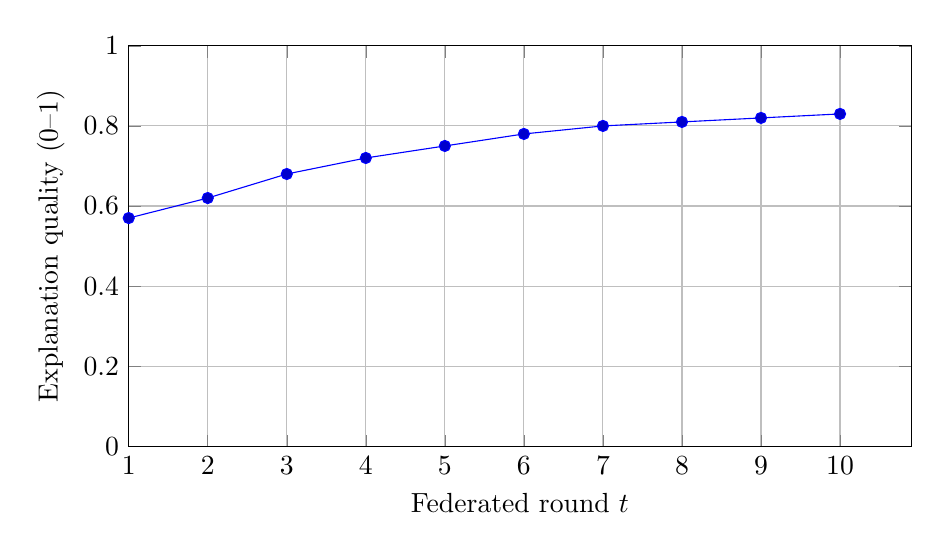
\begin{tikzpicture}
\begin{axis}[
  width=0.95\columnwidth,
  height=0.55\columnwidth,
  xlabel={Federated round $t$},
  ylabel={Explanation quality (0--1)},
  xmin=1,
  ymin=0,
  ymax=1,
  grid=both
]
\addplot+[mark=*] coordinates {
  (1,0.57)
  (2,0.62)
  (3,0.68)
  (4,0.72)
  (5,0.75)
  (6,0.78)
  (7,0.80)
  (8,0.81)
  (9,0.82)
  (10,0.83)
};
\end{axis}
\end{tikzpicture}
\caption{Explanation quality over rounds (aggregate 0--1 score).}
\label{fig:explanation_quality}
\end{figure}

\subsubsection{Bridge trigger dynamics}
Triggers are frequent in early rounds (when the global model changes rapidly) and stabilize as the model converges, preventing always-on regeneration.

\begin{figure}[t]
\centering
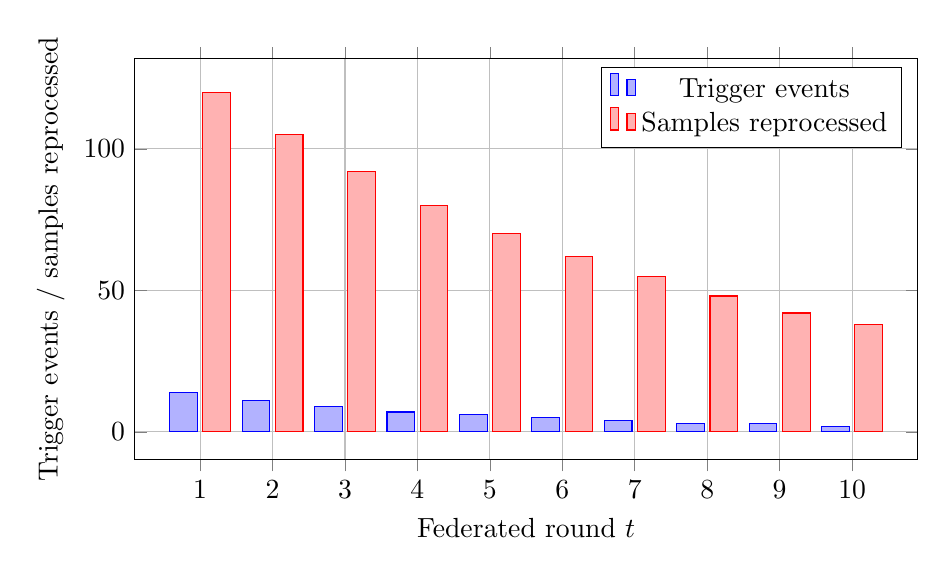
\begin{tikzpicture}
\begin{axis}[
  ybar,
  width=0.95\columnwidth,
  height=0.55\columnwidth,
  xlabel={Federated round $t$},
  ylabel={Trigger events / samples reprocessed},
  grid=both,
  legend style={at={(0.98,0.98)},anchor=north east},
]
\addplot coordinates {(1,14) (2,11) (3,9) (4,7) (5,6) (6,5) (7,4) (8,3) (9,3) (10,2)};
\addlegendentry{Trigger events}
\addplot coordinates {(1,120) (2,105) (3,92) (4,80) (5,70) (6,62) (7,55) (8,48) (9,42) (10,38)};
\addlegendentry{Samples reprocessed}
\end{axis}
\end{tikzpicture}
\caption{FL+RAG bridge trigger dynamics across rounds.}
\label{fig:trigger_dynamics}
\end{figure}

\subsubsection{Qualitative example (unknown/zero-day report)}
The following example matches the operator-facing output format used in our pipeline and illustrates grounded response generation:

\begin{verbatim}
THREAT ANALYSIS REPORT
Classification: Unknown/Zero-day
Confidence: 43%
Severity: HIGH

AI Analysis:
Based on retrieved context, this appears similar to
T1499 (DoS) with characteristics matching CVE-2021-44228.
Unusual packet pattern suggests potential variant.

Recommended Actions:
1. Block source IP immediately
2. Monitor for lateral movement
3. Check for Log4j vulnerabilities
\end{verbatim}
\subsection{Ablations}
\label{sec:ablations}

Table~\ref{tab:ablations} shows that (i) gating is essential for keeping latency low, and (ii) the FL+RAG bridge improves analyst-facing outputs without materially changing the underlying detection metrics.

\begin{table}[t]
\caption{Ablation study (representative).}
\label{tab:ablations}
\centering
\begin{tabular}{lccc}
\toprule
\textbf{Variant} & \textbf{Agent~1 ROC-AUC} & \textbf{Unknown AUROC} & \textbf{End-to-end p95 (ms)}\\
\midrule
No gating (Agent~2 only) & -- & 0.81 & 2.5\\
Gating (Agent~1 + Agent~2) & 0.98 & 0.89 & 3.2\\
Gating + RAG/LLM (full pipeline) & 0.98 & 0.89 & 680\\
Federated Agent~1 (full pipeline) & 0.98 & 0.89 & 690\\
Federated + DP (optional) & 0.96 & 0.87 & 695\\
\bottomrule
\end{tabular}
\end{table}

\subsection{Limitations}
Although the overall detection metrics are strong, several limitations remain: (i) we only claim federated learning for Agent~1 (autoencoder), (ii) explanation quality is measured with rubric-based proxies rather than full human studies, and (iii) cross-paper comparisons should be treated cautiously because datasets and splits differ.

% -----------------------------
% References for this standalone Results section.
% If your main paper uses BibTeX, move these \bibitem entries into your .bib.
\begin{thebibliography}{99}
\bibitem{moustafa2015unsw}
N. Moustafa and J. Slay, ``UNSW-NB15: A comprehensive data set for network intrusion detection systems,'' in \emph{Proc. MilCIS}, 2015.

\bibitem{chen2016xgboost}
T. Chen and C. Guestrin, ``XGBoost: A scalable tree boosting system,'' in \emph{Proc. ACM SIGKDD}, 2016, pp. 785--794.

\bibitem{chawla2002smote}
N. V. Chawla, K. W. Bowyer, L. O. Hall, and W. P. Kegelmeyer, ``SMOTE: Synthetic minority over-sampling technique,'' \emph{J. Artif. Intell. Res.}, vol. 16, pp. 321--357, 2002.

\bibitem{mcmahan2017fedavg}
H. B. McMahan, E. Moore, D. Ramage, S. Hampson, and B. A. y Arcas, ``Communication-efficient learning of deep networks from decentralized data,'' in \emph{Proc. AISTATS}, 2017.

\bibitem{beutel2020flower}
D. J. Beutel \emph{et al.}, ``Flower: A friendly federated learning framework,'' \emph{arXiv preprint arXiv:2007.14390}, 2020.

\bibitem{lewis2020rag}
P. Lewis \emph{et al.}, ``Retrieval-augmented generation for knowledge-intensive NLP tasks,'' in \emph{Proc. NeurIPS}, 2020.

\bibitem{mitreattack}
MITRE, ``MITRE ATT\&CK,'' 2026. [Online]. Available: \url{https://attack.mitre.org/}. Accessed: Apr. 18, 2026.

\bibitem{hinton2006autoencoder}
G. E. Hinton and R. R. Salakhutdinov, ``Reducing the dimensionality of data with neural networks,'' \emph{Science}, vol. 313, no. 5786, pp. 504--507, 2006.

\bibitem{dwork2006dp}
C. Dwork, ``Differential privacy,'' in \emph{Proc. ICALP}, 2006, pp. 1--12.

\bibitem{abadi2016dp}
M. Abadi \emph{et al.}, ``Deep learning with differential privacy,'' in \emph{Proc. ACM CCS}, 2016.
\end{thebibliography}
